\documentclass[
    xcolor={svgnames,dvipsnames},
    hyperref={colorlinks, citecolor=DeepPink4, linkcolor=DarkRed, urlcolor=DarkBlue}
    ]{beamer}  % for hardcopy add 'trans'


\mode<presentation>
{
  \usetheme{Pittsburgh}
  % or ...
  \setbeamercovered{transparent}
  % or whatever (possibly just delete it)
}

\usefonttheme{professionalfonts}
%\usepackage[english]{babel}
% or whatever
%\usepackage[latin1]{inputenc}
% or whatever
%\usepackage{times}
%\usepackage[T1]{fontenc}
% Or whatever. Note that the encoding and the font should match. If T1
% does not look nice, try deleting the line with the fontenc.

%\usepackage{fontspec}
%\setmonofont{CMU Typewriter Text}
%\setmonofont{Consolas}

%%%%%%%%%%%%%%%%%%%%%% start my preamble %%%%%%%%%%%%%%%%%%%%%%

\addtobeamertemplate{navigation symbols}{}{%
    \usebeamerfont{footline}%
    \usebeamercolor[fg]{footline}%
    \hspace{1em}%
    \insertframenumber/\inserttotalframenumber
}


\usepackage{graphicx}
\usepackage{amsmath, amssymb, amsthm}
\usepackage{bbm}
\usepackage{mathrsfs}
\usepackage{xcolor}
\usepackage{fancyvrb}

% Quotes at start of chapters / sections
\usepackage{epigraph}  
%\renewcommand{\epigraphflush}{flushleft}
%\renewcommand{\sourceflush}{flushleft}
\renewcommand{\epigraphwidth}{6in}

%% Fonts

%\usepackage[T1]{fontenc}
\usepackage{mathpazo}
%\usepackage{fontspec}
%\defaultfontfeatures{Ligatures=TeX}
%\setsansfont[Scale=MatchLowercase]{DejaVu Sans}
%\setmonofont[Scale=MatchLowercase]{DejaVu Sans Mono}
%\setmathfont{Asana Math}
%\setmainfont{Optima}
%\setmathrm{Optima}
%\setboldmathrm[BoedFont={Optima ExtraBlack}]{Optima Bold}

% Some colors

\definecolor{aquamarine}{RGB}{69,139,116}
\definecolor{midnightblue}{RGB}{25,25,112}
\definecolor{darkslategrey}{RGB}{47,79,79}
\definecolor{darkorange4}{RGB}{139,90,0}
\definecolor{dogerblue}{RGB}{24,116,205}
\definecolor{blue2}{RGB}{0,0,238}
\definecolor{bg}{rgb}{0.95,0.95,0.95}
\definecolor{DarkOrange1}{RGB}{255,127,0}
\definecolor{ForestGreen}{RGB}{34,139,34}
\definecolor{DarkRed}{RGB}{139, 0, 0}
\definecolor{DarkBlue}{RGB}{0, 0, 139}
\definecolor{Blue}{RGB}{0, 0, 255}
\definecolor{Brown}{RGB}{165,42,42}


\setlength{\parskip}{1.5ex plus0.5ex minus0.5ex}

%\renewcommand{\baselinestretch}{1.05}
%\setlength{\parskip}{1.5ex plus0.5ex minus0.5ex}
%\setlength{\parindent}{0pt}

% Typesetting code
\definecolor{bg}{rgb}{0.95,0.95,0.95}
\usepackage{minted}
\setminted{mathescape, frame=lines, framesep=3mm}
\usemintedstyle{friendly}
%\newminted{python}{}
%\newminted{c}{mathescape,frame=lines,framesep=4mm,bgcolor=bg}
%\newminted{java}{mathescape,frame=lines,framesep=4mm,bgcolor=bg}
%\newminted{julia}{mathescape,frame=lines,framesep=4mm,bgcolor=bg}
%\newminted{ipython}{mathescape,frame=lines,framesep=4mm,bgcolor=bg}

% Typesetting code
\definecolor{bg}{rgb}{0.95,0.95,0.95}
\usepackage{minted}
\usemintedstyle{friendly}
\newminted{python}{mathescape,frame=lines,framesep=4mm,bgcolor=bg}
\newminted{ipython}{mathescape,frame=lines,framesep=4mm,bgcolor=bg}
\newminted{julia}{mathescape,frame=lines,framesep=4mm,bgcolor=bg}
\newminted{c}{mathescape,linenos=true}
\renewcommand{\theFancyVerbLine}{\sffamily
    \textcolor[rgb]{0.5,0.5,1.0}{\scriptsize {\arabic{FancyVerbLine}}}}


\newcommand{\Fact}{\textcolor{Brown}{\bf Fact. }}
\newcommand{\Facts}{\textcolor{Brown}{\bf Facts }}
\newcommand{\keya}{\textcolor{turquois4}{\bf Key Idea. }}
\newcommand{\Factnodot}{\textcolor{Brown}{\bf Fact }}
\newcommand{\Eg}{\textcolor{ForestGreen}{Example. }}
\newcommand{\Egs}{\textcolor{ForestGreen}{Examples. }}
\newcommand{\Ex}{{\bf Ex. }}



\renewcommand{\theFancyVerbLine}{\sffamily
    \textcolor[rgb]{0.5,0.5,1.0}{\scriptsize {\arabic{FancyVerbLine}}}}

\newcommand{\navy}[1]{\textcolor{Blue}{\bf #1}}
\newcommand{\brown}[1]{\textcolor{Brown}{\sf #1}}
\newcommand{\green}[1]{\textcolor{ForestGreen}{\sf #1}}
\newcommand{\blue}[1]{\textcolor{Blue}{\sf #1}}
\newcommand{\navymth}[1]{\textcolor{Blue}{#1}}
\newcommand{\emp}[1]{\textcolor{DarkOrange1}{\bf #1}}
\newcommand{\red}[1]{\textcolor{Red}{\bf #1}}

% Symbols, redefines, etc.

\newcommand{\code}[1]{\texttt{#1}}

\newcommand{\argmax}{\operatornamewithlimits{argmax}}
\newcommand{\argmin}{\operatornamewithlimits{argmin}}

\DeclareMathOperator{\cl}{cl}
\DeclareMathOperator{\interior}{int}
\DeclareMathOperator{\Prob}{Prob}
\DeclareMathOperator{\determinant}{det}
\DeclareMathOperator{\trace}{trace}
\DeclareMathOperator{\Span}{span}
\DeclareMathOperator{\rank}{rank}
\DeclareMathOperator{\cov}{cov}
\DeclareMathOperator{\corr}{corr}
\DeclareMathOperator{\var}{var}
\DeclareMathOperator{\mse}{mse}
\DeclareMathOperator{\se}{se}
\DeclareMathOperator{\row}{row}
\DeclareMathOperator{\col}{col}
\DeclareMathOperator{\range}{rng}
\DeclareMathOperator{\dimension}{dim}
\DeclareMathOperator{\bias}{bias}


% mics short cuts and symbols
\newcommand{\st}{\ensuremath{\ \mathrm{s.t.}\ }}
\newcommand{\setntn}[2]{ \{ #1 : #2 \} }
\newcommand{\cf}[1]{ \lstinline|#1| }
\newcommand{\fore}{\therefore \quad}
\newcommand{\tod}{\stackrel { d } {\to} }
\newcommand{\toprob}{\stackrel { p } {\to} }
\newcommand{\toms}{\stackrel { ms } {\to} }
\newcommand{\eqdist}{\stackrel {\textrm{ \scriptsize{d} }} {=} }
\newcommand{\iidsim}{\stackrel {\textrm{ {\sc iid }}} {\sim} }
\newcommand{\1}{\mathbbm 1}
\newcommand{\dee}{\,{\rm d}}
\newcommand{\given}{\, | \,}
\newcommand{\la}{\langle}
\newcommand{\ra}{\rangle}

\newcommand{\boldA}{\mathbf A}
\newcommand{\boldB}{\mathbf B}
\newcommand{\boldC}{\mathbf C}
\newcommand{\boldD}{\mathbf D}
\newcommand{\boldM}{\mathbf M}
\newcommand{\boldP}{\mathbf P}
\newcommand{\boldQ}{\mathbf Q}
\newcommand{\boldI}{\mathbf I}
\newcommand{\boldX}{\mathbf X}
\newcommand{\boldY}{\mathbf Y}
\newcommand{\boldZ}{\mathbf Z}

\newcommand{\bSigmaX}{ {\boldsymbol \Sigma_{\hboldbeta}} }
\newcommand{\hbSigmaX}{ \mathbf{\hat \Sigma_{\hboldbeta}} }

\newcommand{\RR}{\mathbbm R}
\newcommand{\NN}{\mathbbm N}
\newcommand{\PP}{\mathbbm P}
\newcommand{\EE}{\mathbbm E \,}
\newcommand{\XX}{\mathbbm X}
\newcommand{\ZZ}{\mathbbm Z}
\newcommand{\QQ}{\mathbbm Q}

\newcommand{\fF}{\mathcal F}
\newcommand{\dD}{\mathcal D}
\newcommand{\lL}{\mathcal L}
\newcommand{\gG}{\mathcal G}
\newcommand{\hH}{\mathcal H}
\newcommand{\nN}{\mathcal N}
\newcommand{\pP}{\mathcal P}




\title{Scientific Computing in Economics and Finance\\
    Past, Present and Future}

\author{John Stachurski}
\institute{Tokyo College and Australian National University}


\date{April 25th 2025}


\begin{document}

\begin{frame}
  \titlepage
\end{frame}





\section{Introduction}


\begin{frame}
    \frametitle{What is economics?}

    The study of allocation of scarce resources among competing 
    human users.

            \vspace{0.3em}
            \vspace{0.3em}
            \vspace{0.3em}
    \pause

    Combines:

    \begin{itemize}
        \item Social science (history, politics, etc.)
            \vspace{0.3em}
            \vspace{0.3em}
            \vspace{0.3em}
        \item Data science (statistics, machine learning)
            \vspace{0.3em}
            \vspace{0.3em}
            \vspace{0.3em}
        \item Mathematical modeling
            \vspace{0.3em}
            \vspace{0.3em}
            \vspace{0.3em}
        \item Computer science
    \end{itemize}


\end{frame}

\begin{frame}
    \frametitle{What do economists do?}

    Study economic phenomena and trends

            \vspace{0.3em}
            \vspace{0.3em}
            \vspace{0.3em}
    \Egs

    \begin{itemize}
        \item Booms and busts
            \vspace{0.3em}
            \vspace{0.3em}
            \vspace{0.3em}
        \item Long run growth
            \vspace{0.3em}
            \vspace{0.3em}
            \vspace{0.3em}
        \item Concentration in industries
            \vspace{0.3em}
            \vspace{0.3em}
            \vspace{0.3em}
        \item Changes in the distribution of wealth
    \end{itemize}

\end{frame}

\begin{frame}
    
    \Eg Long run trends in wealth inequality

    \begin{figure}
        \centering
        \scalebox{.5}{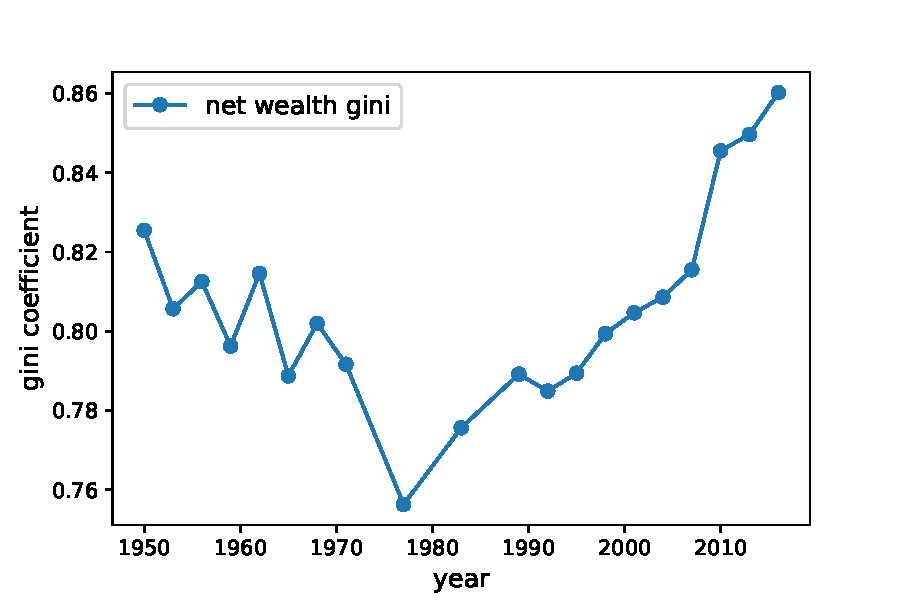
\includegraphics{gini_lorenz_us_3.pdf}}
    \end{figure}


\end{frame}

\begin{frame}
    \frametitle{Practical tasks}

    \begin{itemize}
        \item Design pricing mechanisms for Amazon
            \vspace{0.3em}
            \vspace{0.3em}
            \vspace{0.3em}
        \item Set interest rates at the BOJ
            \vspace{0.3em}
            \vspace{0.3em}
            \vspace{0.3em}
        \item Assess tax policies
            \vspace{0.3em}
            \vspace{0.3em}
            \vspace{0.3em}
        \item Advise on competition policy 
            \vspace{0.3em}
            \vspace{0.3em}
            \vspace{0.3em}
        \item Assess pension plans
            \vspace{0.3em}
            \vspace{0.3em}
            \vspace{0.3em}
        \item Study the impact of COVID / COVID relief policy
    \end{itemize}


\end{frame}

\begin{frame}
    
    Many problems addressed by economists are quantitative

            \vspace{0.3em}
            \vspace{0.3em}

    \Egs 
    %
    \begin{itemize}
        \item How will a 10\% increase in the top income tax rate affect GDP
            over the next decade?
            \vspace{0.3em}
            \vspace{0.3em}
        \item How will a two year increase in the retirement age affect
            government debt?
            \vspace{0.3em}
            \vspace{0.3em}
        \item What will be the impact of a 25 BPS $\uparrow$ in the federal
            funds rate on unemployment next year?
    \end{itemize}

            \vspace{0.3em}
            \vspace{0.3em}

    \begin{center}
        Quantitative problems require mathematical/computational modeling
    \end{center}


\end{frame}


\begin{frame}
    \frametitle{Basic research also requires mathematical modeling}

    \pause

    \brown{The goal of the scientist is to comprehend the phenomena of the
    universe that he observes around him.}

            \vspace{0.3em}
    \brown{To prove that he understands he must be able to predict.}

            \vspace{0.3em}
    \brown{To predict quantitatively one must have a mechanism for producing
    numbers.}

            \vspace{0.3em}
    \brown{This necessarily entails a mathematical model.}

            \vspace{0.3em}
            \vspace{0.3em}
            \vspace{0.3em}
     -- Richard Bellman (1920 -- 1984)

\end{frame}

\begin{frame}
    \frametitle{How should economists build models?}

    Why is economics different to astrophysics, chemistry, etc.?
            \vspace{0.3em}
            \vspace{0.3em}
            \vspace{0.3em}

    \begin{itemize}
        \item Economic processes are nonstationary (no immutable laws)
            \vspace{0.3em}
            \vspace{0.3em}
            \vspace{0.3em}
        \item Economic outcomes depend on human choices
            \vspace{0.3em}
            \vspace{0.3em}
            \vspace{0.3em}
        \item Human choices depend on beliefs, incentives, etc.
    \end{itemize}


    %\Eg The Lucas critique: it is naive to try to predict the effects
        %of a change in economic policy entirely on the basis of relationships
        %observed in historical data

\end{frame}

\begin{frame}
    \frametitle{Example: the cobweb model}

    An ``old'' economic model

    \begin{itemize}
        \item Benner (1876)
        \item Haas and Ezekil (1926)
        \item Ricci (1930)
        \item Kaldor (1934, 1938)
        \item Ezekil (1938)
        \item Harlow (1960)
        \item Rosen, Murphy, and Scheinkman (1994)
    \end{itemize}

\end{frame}

\begin{frame}
    
    \begin{figure}
        \centering
        \scalebox{.56}{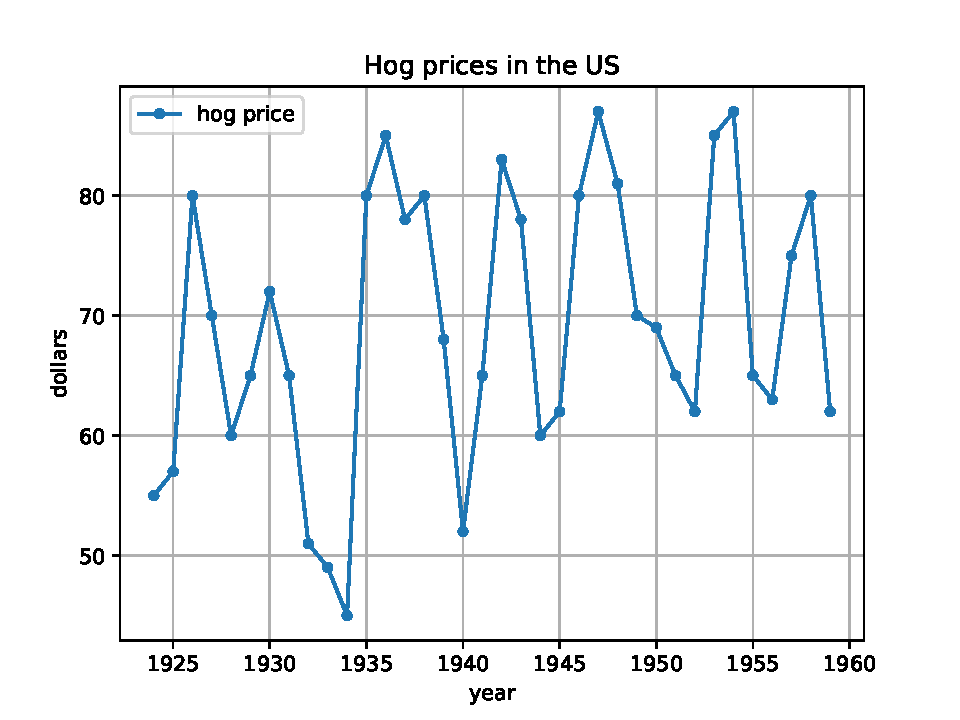
\includegraphics{hog_prices.pdf}}
    \end{figure}

\end{frame}


%\begin{frame}

    %Ordinary models of supply and demand don't generate these cycles.

    %\begin{itemize}
        %\item find $p$ and $q$ from $q^d(p) = q^s(p)$
    %\end{itemize}

    %\begin{figure}
        %\centering
        %\scalebox{.42}{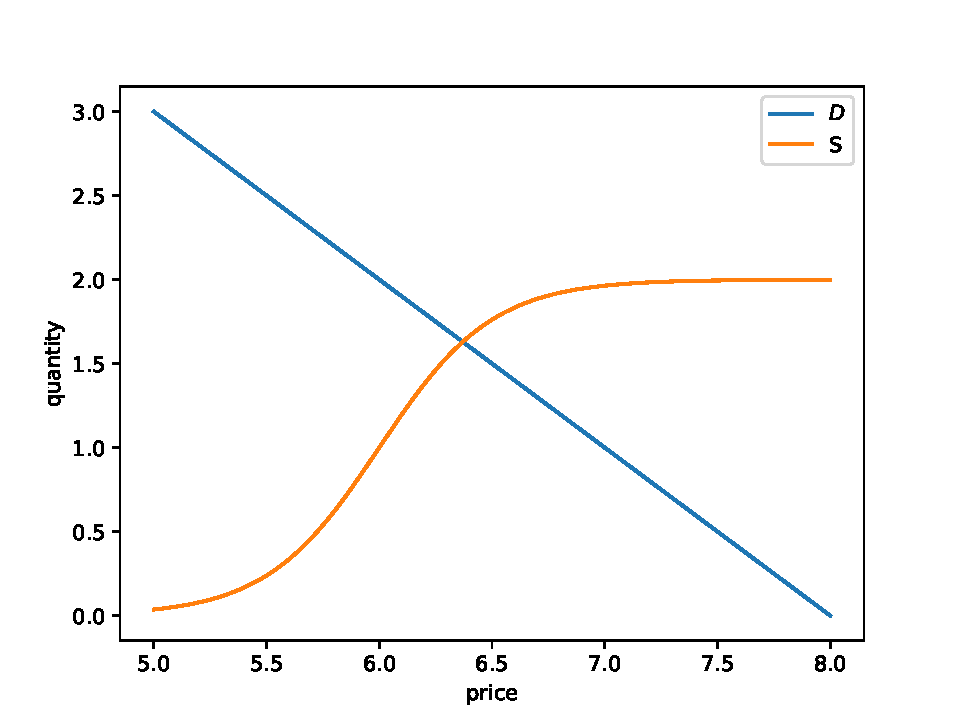
\includegraphics{hog_supply_demand.pdf}}
    %\end{figure}
    

%\end{frame}

\begin{frame}
    
    Hypotheses: 

    \begin{itemize}
        \item Farmers need time to raise hogs (say, one ``period'')
            \vspace{0.3em}
        \item Farmers forecast future prices using current prices
    \end{itemize}

    Outcomes:

    \begin{enumerate}
        \item Suppose price is currently high
            \vspace{0.3em}
        \item Farmers $\uparrow$ capacity, shift towards hog production
            \vspace{0.3em}
        \item Next period, high supply floods the market, prices $\downarrow$
            \vspace{0.3em}
        \item Seeing this low price, farmers $\downarrow$ capacity
            \vspace{0.3em}
        \item Next period, supply is low and prices $\uparrow$ ...
    \end{enumerate}

\end{frame}

\begin{frame}

    In this scenario,
    
    $$
        q^d(p_t) = q^s(p^e_{t-1})
    $$

    \begin{itemize}
        \item $p^e_{t-1}$ is the \textbf{expected} time $t$ price, formed at $t-1$
    \end{itemize}

    \vspace{1em}
    \vspace{1em}

    But how to farmers form expectations?

\end{frame}

\begin{frame}
    
    First guess:
    %
    \begin{equation*}
        p^e_{t-1} = p_{t-1}
    \end{equation*}

    So now we have

    $$
        q^d(p_t) = q^s(p_{t-1})
    $$

    Solving for $p_t$ gives

    $$
        p_t = f(p_{t-1})
        \quad \text{where} \quad
        f(p) = (q^d)^{-1} (q^s(p))
    $$


    Now let's simulate...

\end{frame}

%\begin{frame}
    
    %\begin{figure}
        %\centering
        %\scalebox{.56}{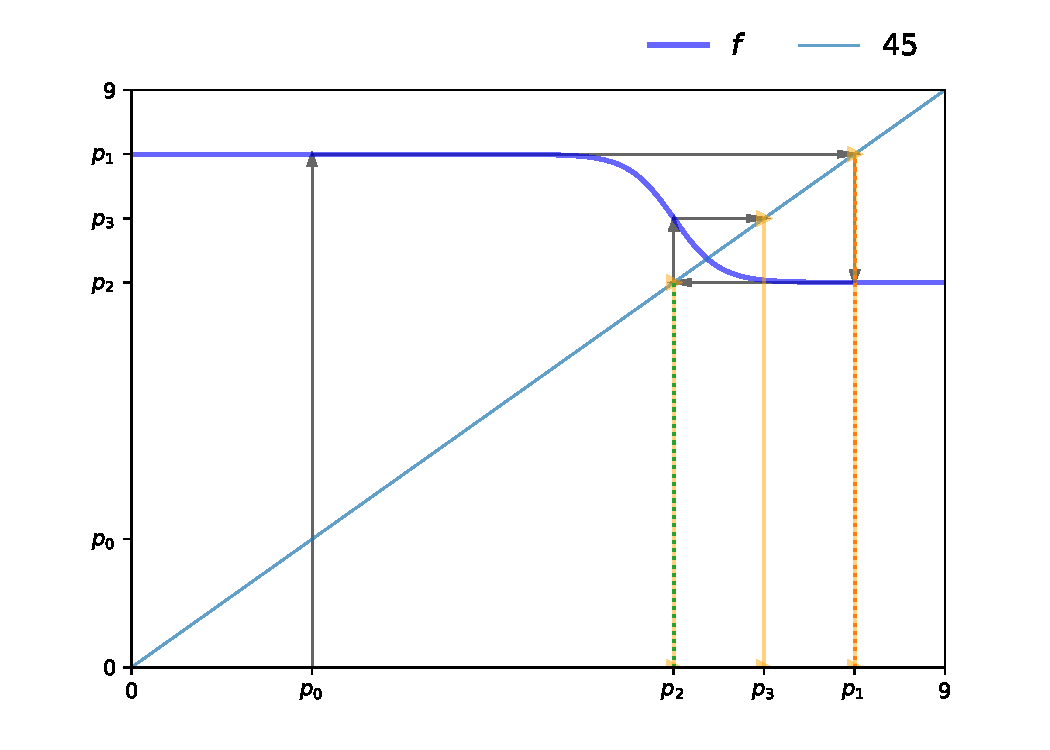
\includegraphics{hog_45.pdf}}
    %\end{figure}

%\end{frame}

\begin{frame}
    
    \begin{figure}
        \centering
        \scalebox{.56}{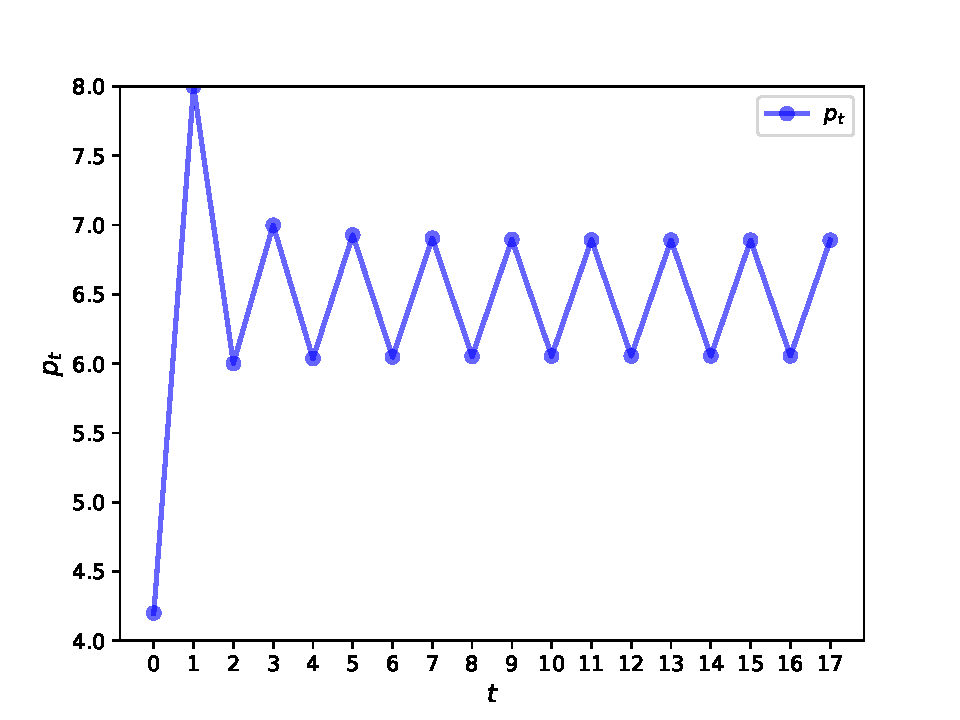
\includegraphics{hog_backward_ts0.pdf}}
    \end{figure}

\end{frame}

\begin{frame}
    
    \begin{figure}
        \centering
        \scalebox{.56}{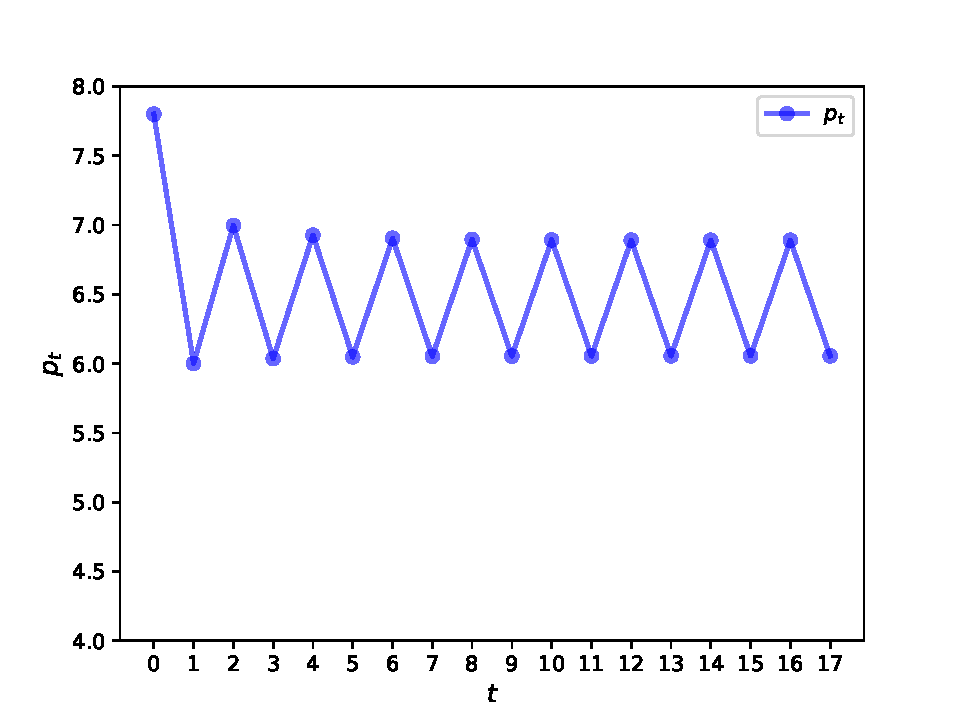
\includegraphics{hog_backward_ts1.pdf}}
    \end{figure}

\end{frame}



\begin{frame}
    
    \begin{figure}
        \centering
        \scalebox{.56}{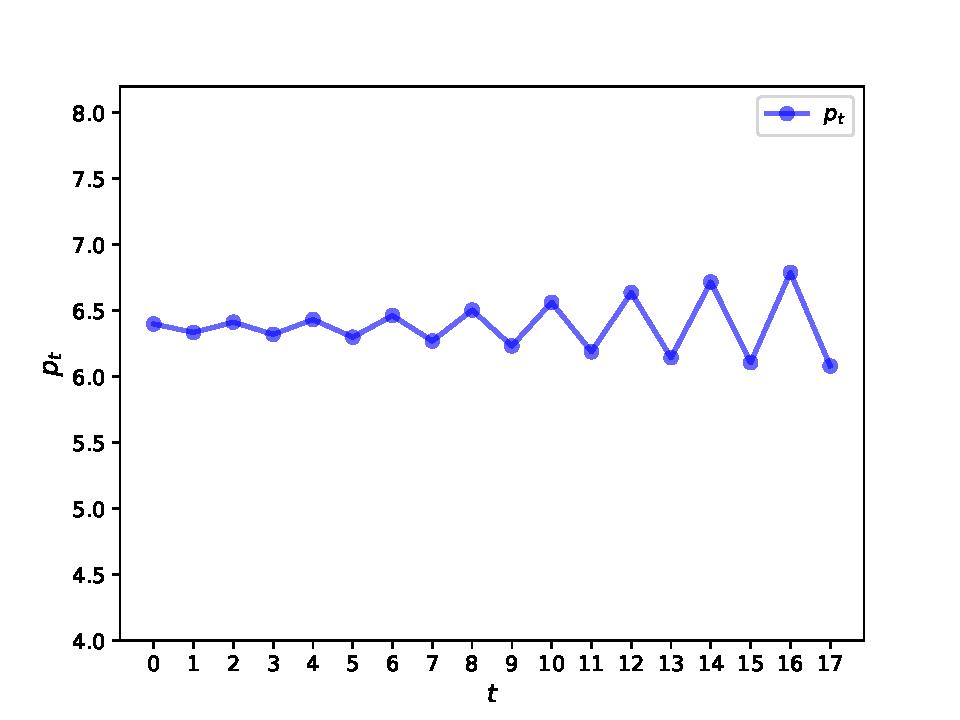
\includegraphics{hog_backward_ts2.pdf}}
    \end{figure}

\end{frame}


\begin{frame}
    
    The model replicates cycles --- but there are problems!

    \vspace{1em}
    \vspace{1em}
    Predictions are \emp{very sensitive} to how we model \emp{expectations}

    \vspace{1em}
    \vspace{1em}
    \vspace{1em}
    \Eg Suppose we switch to $p_{t-1}^e = p^e_{t-2} + \alpha (p_{t-1} - p^e_{t-2}) $ 

    \vspace{1em}
    \vspace{1em}
    \begin{itemize}
        \item Called ``adaptive expectations''
    \end{itemize}

\end{frame}


\begin{frame}
    
    \begin{figure}
        \centering
        \scalebox{.42}{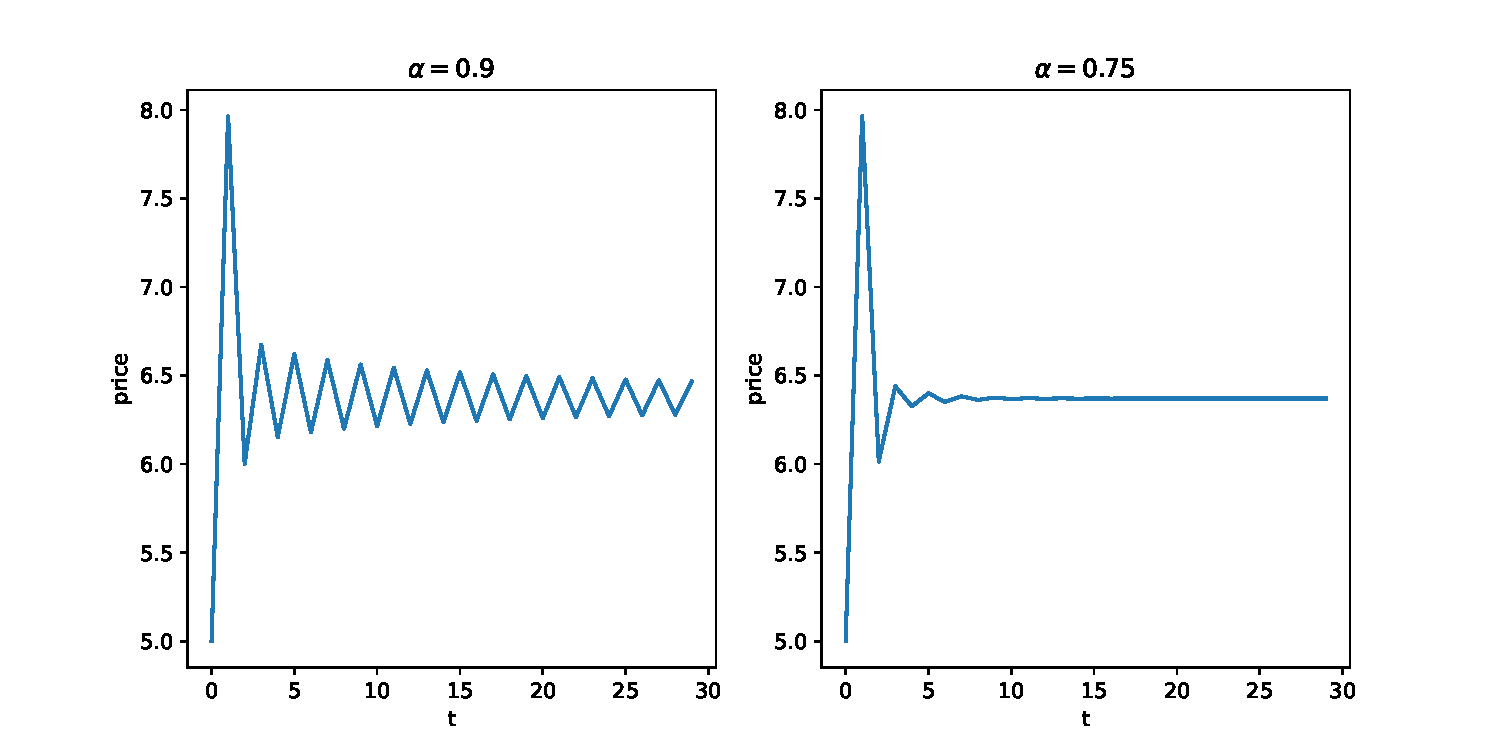
\includegraphics{hog_adaptive.pdf}}
    \end{figure}

\end{frame}


\begin{frame}

    Or we could use ``rational expectations''
    
    \begin{figure}
        \centering
        \scalebox{.46}{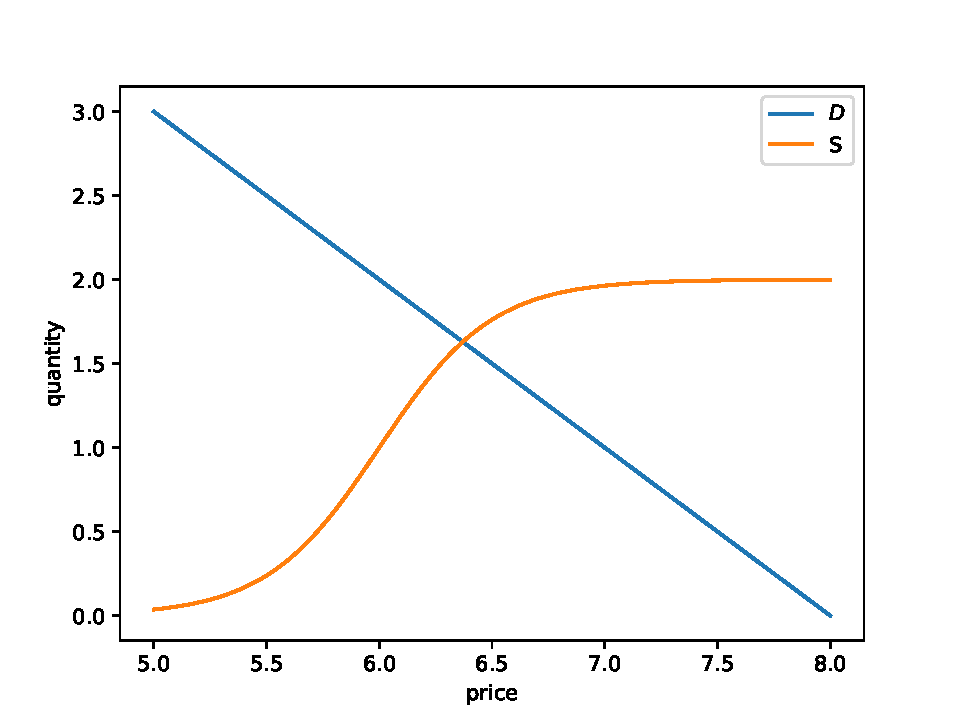
\includegraphics{hog_supply_demand.pdf}}
    \end{figure}

\end{frame}


\begin{frame}

    Lessons:
    %
    \begin{enumerate}
        \item modeling human behavior is essential
            \vspace{1em}
        \item the ``right'' way to model humans is unclear
            \vspace{1em}
        \item predictions are very sensitive to their expectations
            \vspace{1em}
        \item models are nonstationary because the way we predict is
            nonstationary 
    \end{enumerate}
    
        \vspace{1em}
        \vspace{1em}
    Summary: economic modeling is hard -- but we shouldn't give up!

\end{frame}


\begin{frame}
    \frametitle{Scientific computing in economics}

    Anonymous consultant's report on HPC in economics:

    \vspace{0.3em}
    \vspace{0.3em}
    \vspace{0.3em}
    \pause

    \brown{Economists are relative newcomers to the
        field of computational sciences...}

            \vspace{0.3em}
    \brown{Economists have long been influenced by dogmatic tribalism...}

            \vspace{0.3em}
    \brown{It would appear that many (so called) `theories' have been poorly
    (if at all!) proven...}

            \vspace{0.3em}
    \brown{Computational models in economics are still often simplistic...}

\end{frame}


\begin{frame}
    
     \begin{tabular}{cl}  
         \begin{tabular}{c}
           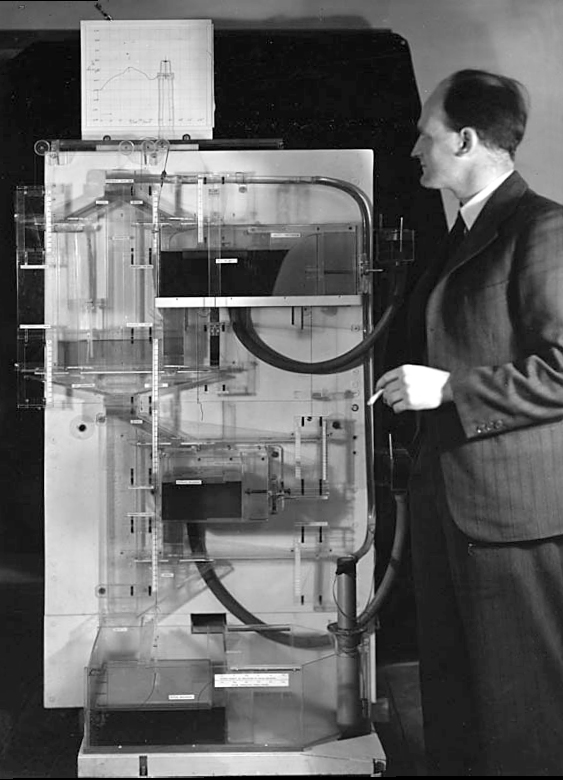
\includegraphics[height=6cm]{moniac.jpg}
           \end{tabular}
           & \begin{tabular}{l}
             \parbox{0.6\linewidth}{%  change the parbox width as appropiate
                Actually economists are pioneers

                (William Phillips, 1949)
             }
         \end{tabular}  \\
    \end{tabular}
    

\end{frame}

\begin{frame}
    \frametitle{Modern scientific computing in economics}

    There are many examples of modern, sophisticated scientific computing in
    economics
            \vspace{0.3em}
            \vspace{0.3em}
            \vspace{0.3em}
    
    \Eg DeepHAM by Jiequn Han, Yucheng Yang, and Weinan E

    \begin{itemize}
        \item heterogeneous agent model
            \vspace{0.3em}
        \item firms and households linked by markets
            \vspace{0.3em}
        \item individual and aggregate risk
            \vspace{0.3em}
        \item general equilibium
            \vspace{0.3em}
        \item NNs to represent human reaction functions
    \end{itemize}

\end{frame}


\begin{frame}

    KS DeepHAM
    
    \begin{figure}
        \centering
        \scalebox{.4}{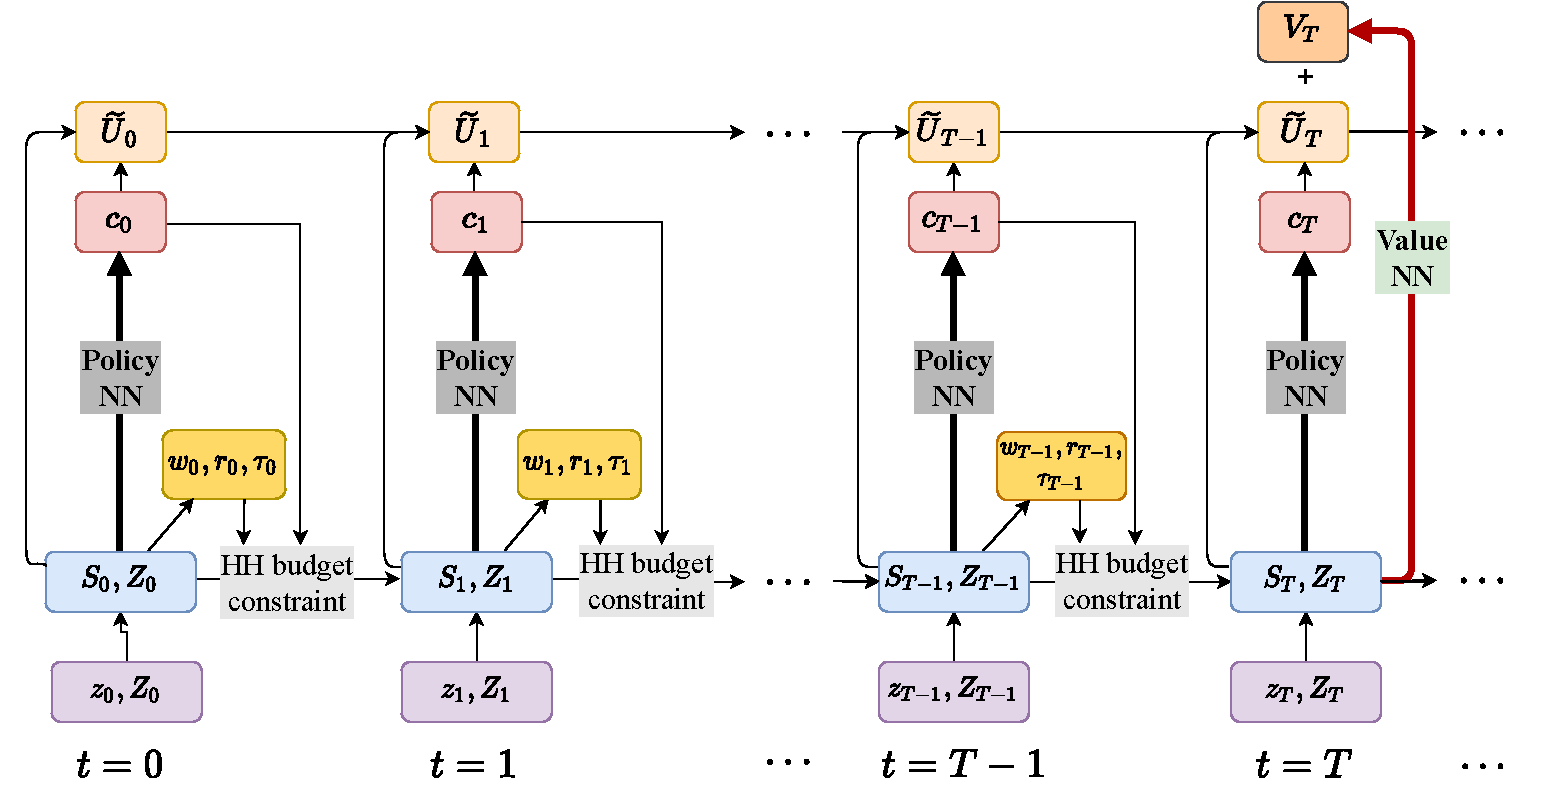
\includegraphics{ks_deep.pdf}}
    \end{figure}

\end{frame}

\begin{frame}
    \frametitle{Trends in scientific computing}

    Technology is advancing rapidly along many dimensions
    %
    \begin{itemize}
        \item improvements to algorithms
    \vspace{0.3em}
        \item new programming languages
    \vspace{0.3em}
        \item new hardware
    \vspace{0.3em}
        \item AI, etc.
    \end{itemize}

    \vspace{0.3em}
    \vspace{0.3em}
    What trends are affecting economics?

    \vspace{0.3em}
    \vspace{0.3em}
    How are they changing economic research?

\end{frame}


\begin{frame}
    \frametitle{Trend 1: Proprietary $\to$ Open Source}
    
    \blue{Proprietary} 
    %
    \begin{itemize}
        \item Excel
        \item MATLAB, Mathematica
        \item STATA, Eviews, SPSS.
    \end{itemize}
    

    \vspace{0.5em}
    \vspace{0.5em}
    \blue{Open Source / Open Standard} 
    
    \begin{itemize}
        \item Python
        \item Julia
        \item R
    \end{itemize}


    \begin{center}
        closed and stable vs open and fast moving
    \end{center}

\end{frame}


\begin{frame}

    Popularity:

    \begin{figure}
       \begin{center}
        \scalebox{1.8}{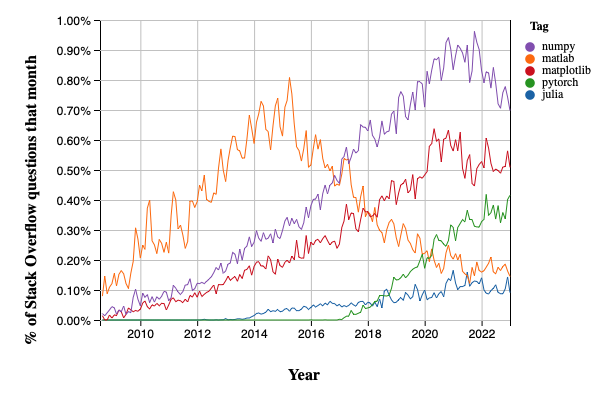
\includegraphics{python_vs_rest.png}}
       \end{center}
    \end{figure}

\end{frame}


\begin{frame}
    \frametitle{Trend 2: Low Level $\to$ High Level}
    
    \blue{Low level} 
    
    \begin{itemize}
        \item C/C++
        \item Fortran
        \item Assembly
    \end{itemize}

    \vspace{1em}

    \blue{High level } 

    \begin{itemize}
        \item Python
        \item Javascript
        \item PHP
    \end{itemize}

\end{frame}


\begin{frame}
    
    \blue{Low level languages} give us control 

    \begin{itemize}
        \item control CPU
        \item control memory
    \end{itemize}

    \vspace{0.5em}
    \vspace{0.5em}
    \vspace{0.5em}

    \blue{High level languages} give us 
    %
    \begin{itemize}
        \item abstraction
        \item automation
        \item flexibility, etc.
    \end{itemize}

\end{frame}




\begin{frame}[fragile]

    \Eg \brown{1 + 1} in assembly

    {\small
    \begin{minted}{as}
pushq   %rbp
movq    %rsp, %rbp
movl    $1, -12(%rbp)
movl    $1, -8(%rbp)
movl    -12(%rbp), %edx
movl    -8(%rbp), %eax
addl    %edx, %eax
movl    %eax, -4(%rbp)
movl    -4(%rbp), %eax
popq    %rbp
    \end{minted}
    }

\end{frame}


\begin{frame}[fragile]

    \Eg \brown{1 + 1} in C

    {\small
    \begin{minted}{c}
#include <stdio.h>
int main() {
    int sum = 1 + 1;
    printf("1 + 1 = %d\n", sum);
    return 0;
}   
    \end{minted}
    }

\end{frame}

\begin{frame}[fragile]

    \Eg \brown{1 + 1} in Python

    {\small
    \begin{minted}{python}
sum = 1 + 1
print("1 + 1 = ", sum)
    \end{minted}
    }

\end{frame}



\begin{frame}

    Trade-offs:
    
    \begin{figure}
        \centering
        \scalebox{.5}{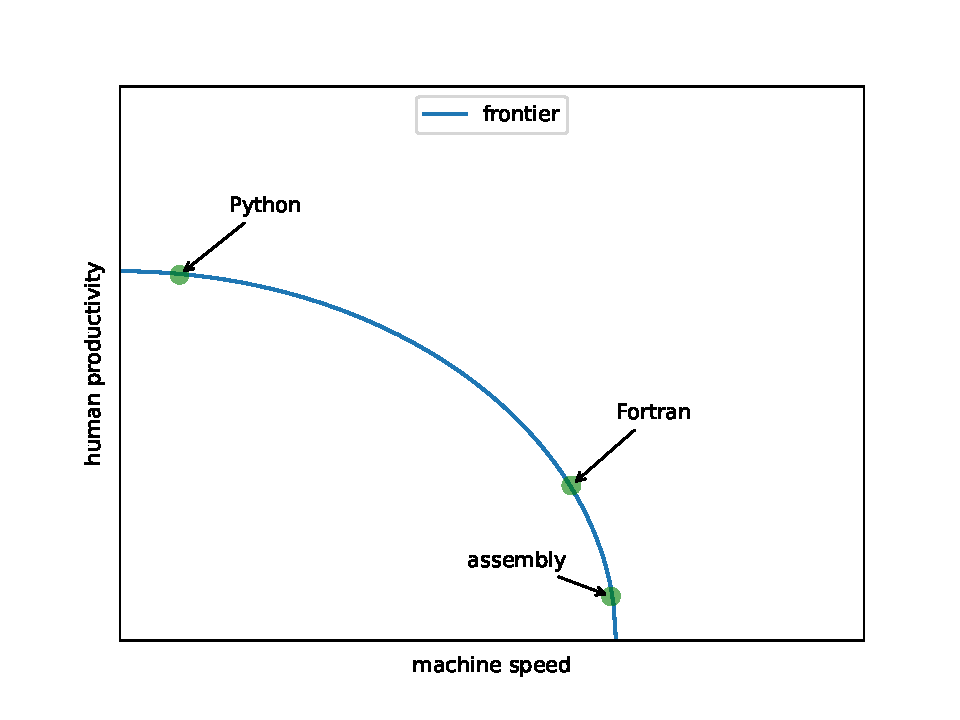
\includegraphics{ppf.pdf}}
    \end{figure}


\end{frame}



\begin{frame}[fragile]

    New trend --- a shifting frontier!

\end{frame}




\begin{frame}
    
    \begin{figure}
        \centering
        \scalebox{.5}{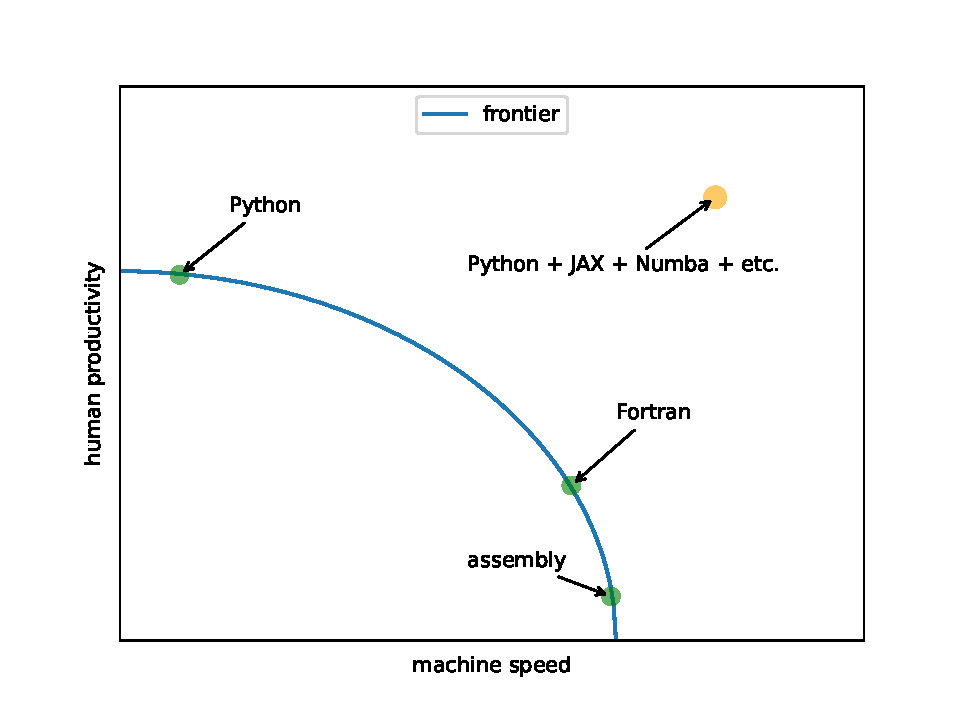
\includegraphics{ppf_plus.pdf}}
    \end{figure}

\end{frame}




\begin{frame}

    \Eg \texttt{Numba} / \texttt{codon} generate fast machine code from Python

    \vspace{0.5em}
    \vspace{0.5em}
    \vspace{0.5em}
    \vspace{0.5em}
    See code at
    %
    \begin{center}
        \url{https://github.com/QuantEcon/tokyo_college_2023/}
    \end{center}

\end{frame}



    

\begin{frame}

    \frametitle{Trend 3: Parallelization}

    CPU frequency (clock speed) growth is slowing

    \begin{figure}
       \begin{center}
        \scalebox{.22}{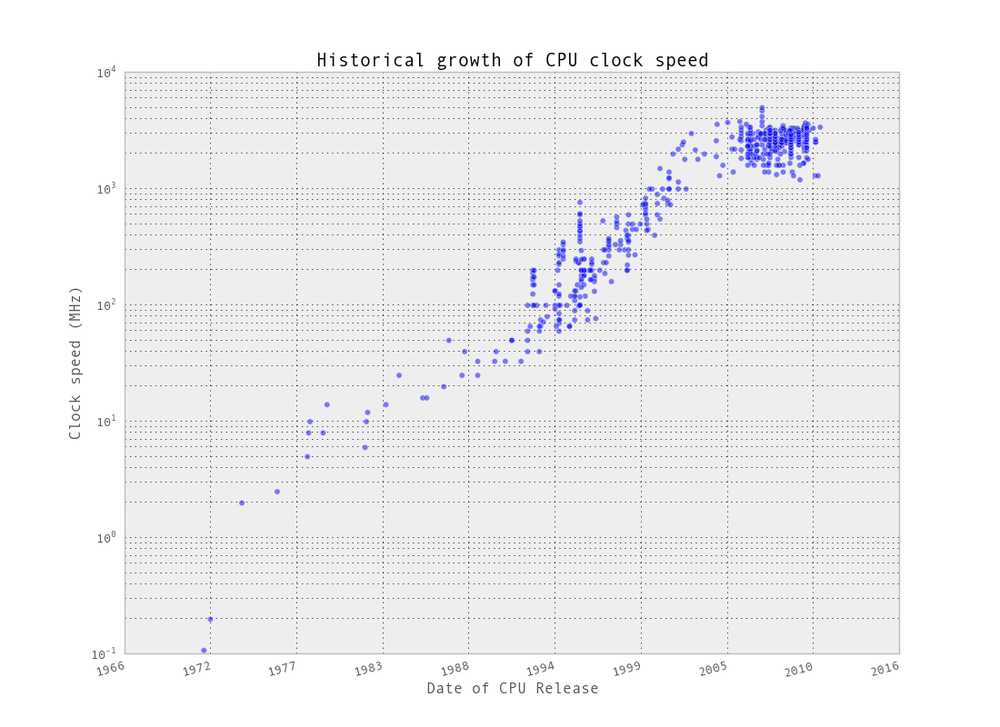
\includegraphics{processor_clock.png}}
       \end{center}
    \end{figure}

\end{frame}



\begin{frame}
    
    Chip makers have responded by developing multi-core processors

    \begin{figure}
       \begin{center}
        \scalebox{.2}{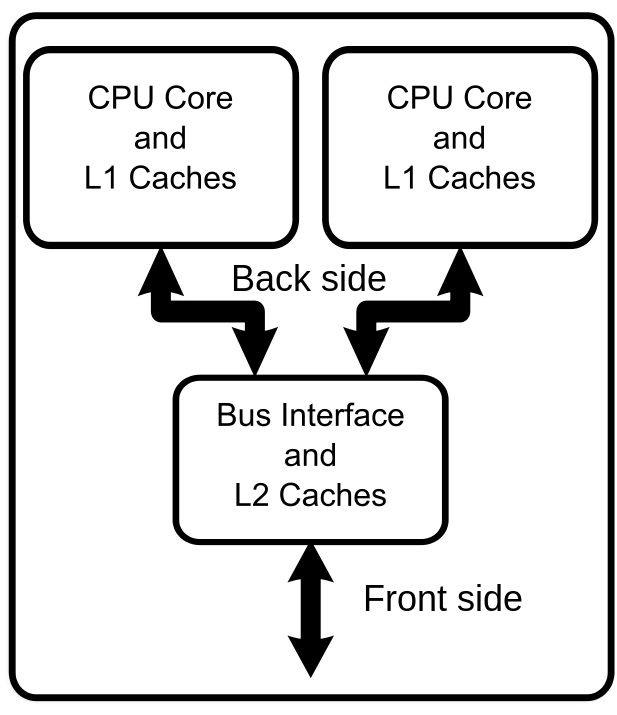
\includegraphics{dual_core.png}}
       \end{center}
    \end{figure}

    Source: Wikipedia


\end{frame}


\begin{frame}

    \navy{GPUs} are becoming increasingly important


    \begin{figure}
       \begin{center}
        \scalebox{.16}{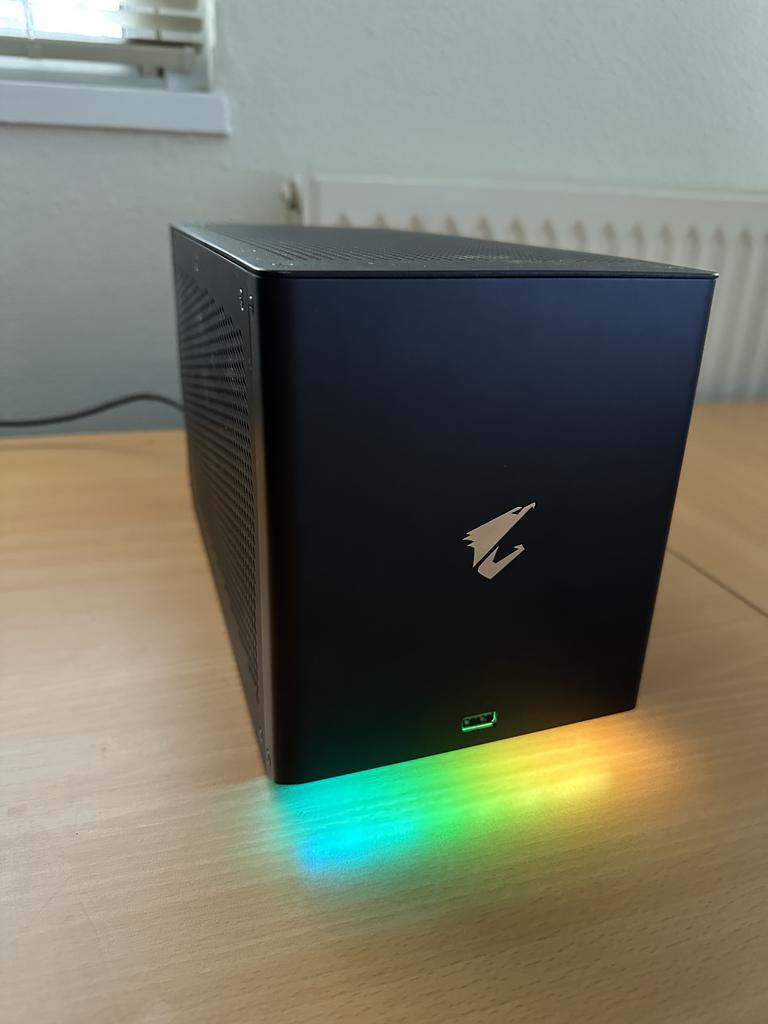
\includegraphics{gpu.jpg}}
       \end{center}
    \end{figure}

    \vspace{0.5em}

    Applications: machine learning, deep learning, etc.
    

\end{frame}


%\begin{frame}
    %\frametitle{Support for Parallelization}
    
    %While scientific computing environments best support parallelization?

        %\vspace{0.5em}
        %\vspace{0.5em}
    %%
    %\begin{itemize}
        %\item Most have some support
        %\vspace{0.5em}
        %\item but which make it easy to harness its power?
    %\end{itemize}

    %\vspace{0.5em}
    %\vspace{0.5em}

    %Current winner:
    %%
    %\begin{itemize}
        %\item Google JAX (Python library)
            %\vspace{0.5em}
    %\end{itemize}

%\end{frame}



\begin{frame}

    \Eg JAX 

    \vspace{0.5em}
    \vspace{0.5em}
    \vspace{0.5em}
    \vspace{0.5em}
    \vspace{0.5em}
    See code at
    %
    \begin{center}
        \url{https://github.com/QuantEcon/tokyo_college_2023/}
    \end{center}

\end{frame}




\begin{frame}
    \frametitle{The limits of computer power}


    Consider optimizing a function via brute force
        
\end{frame}




\begin{frame}
    
    \begin{figure}
       \begin{center}
           \scalebox{.4}{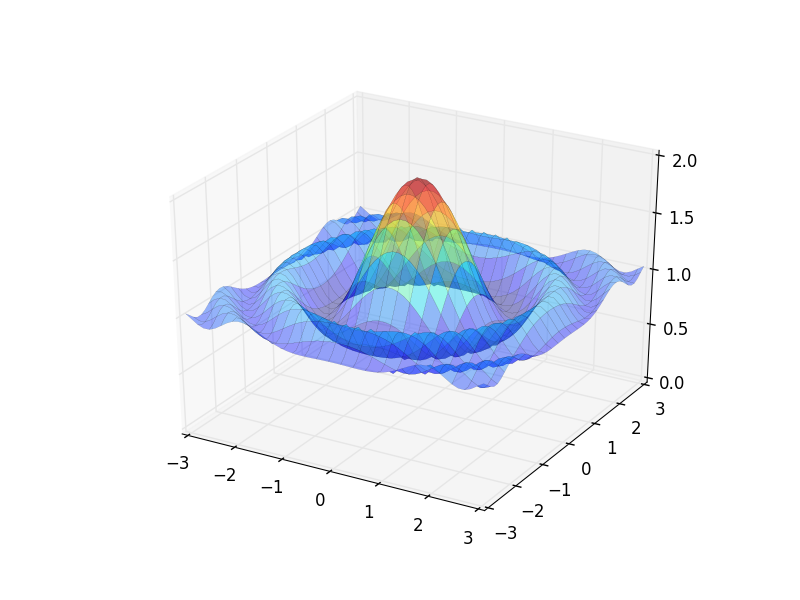
\includegraphics{brute_force_1.png}}
           \caption{The function to maximize}
       \end{center}
    \end{figure}

\end{frame}



\begin{frame}
    
    \begin{figure}
       \begin{center}
           \scalebox{.4}{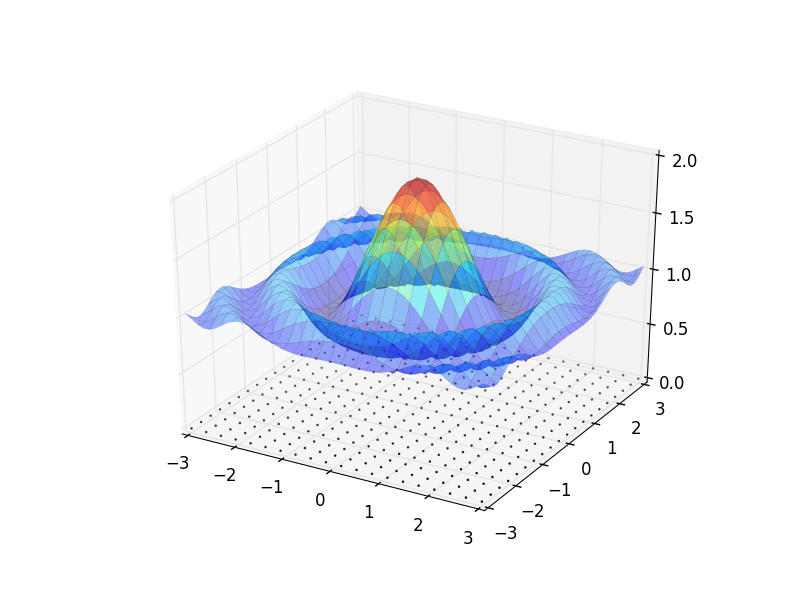
\includegraphics{brute_force_2.png}}
           \caption{Grid of points to evaluate the function at}
       \end{center}
    \end{figure}

\end{frame}

\begin{frame}
    
    \begin{figure}
       \begin{center}
           \scalebox{.4}{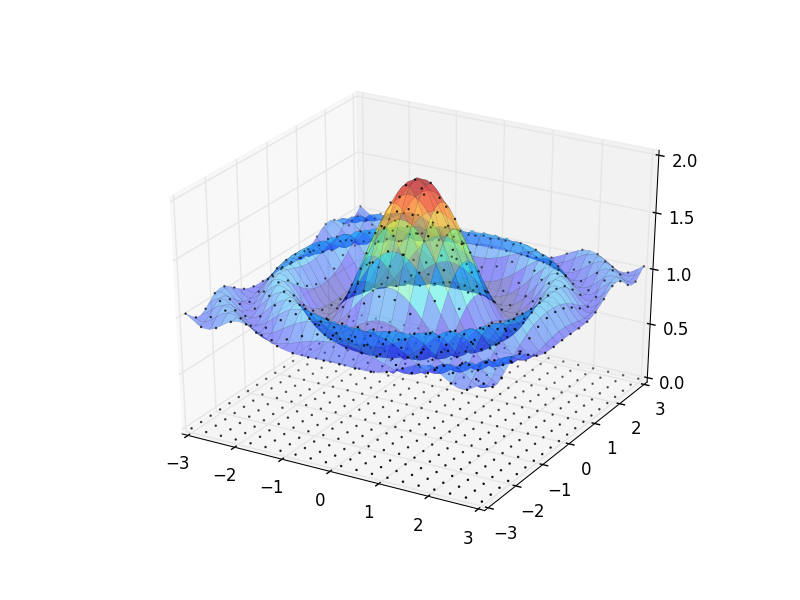
\includegraphics{brute_force_3.png}}
           \caption{Evaluations}
       \end{center}
    \end{figure}

\end{frame}


\begin{frame}
    
    Grid size = $20 \times 20 = 400$

    \vspace{0.5em}
    Outcomes

    \begin{itemize}
        \item function evaluations $= 400$
    \vspace{0.5em}
        \item Time taken $\approx 0$
    \vspace{0.5em}
        \item Max value $= 1.951$
    \vspace{0.5em}
        \item True maximum $= 2$
    \end{itemize}

    \vspace{0.5em}
    \vspace{0.5em}
\end{frame}


\begin{frame}
    
    \begin{figure}
       \begin{center}
           \scalebox{.4}{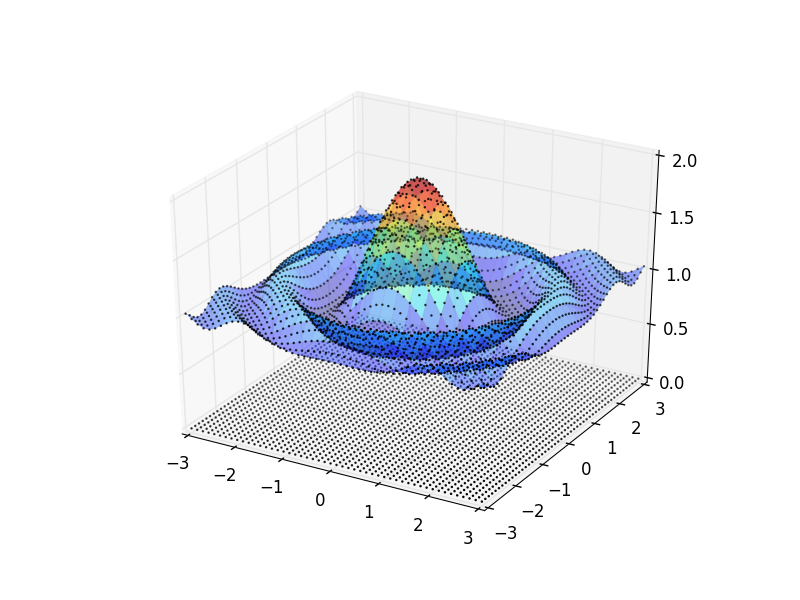
\includegraphics{brute_force_4.png}}
           \caption{$50^2 = 2500$ evaluations}
       \end{center}
    \end{figure}

\end{frame}


\begin{frame}
    
    \begin{itemize}
        \item function evaluations $= 50^2$
    \vspace{0.5em}
        \item Time taken = $101$ microseconds
    \vspace{0.5em}
        \item Max value $= 1.992$
    \vspace{0.5em}
        \item True maximum $= 2$
    \end{itemize}

    \vspace{1em}


\end{frame}


\begin{frame}
    
    But now suppose we hav more choice variables

    \begin{itemize}
        \item 3 vars: $\max_{x_1, x_2, x_3} f(x_1, x_2, x_3)$
        \vspace{0.5em}
        \item 4 vars: $\max_{x_1, x_2, x_3, x_4} f(x_1, x_2, x_3, x_4)$
        \vspace{0.5em}
        \item $\cdots$
    \end{itemize}


\end{frame}

\begin{frame}
    

    If we have 50 grid points per variable and 
    
    \begin{itemize}
        \item 2 variables then evaluations $=50^2 = 2500$
        \vspace{0.5em}
        \item 3 variables then evaluations $=50^3 = 125,000$
        \vspace{0.5em}
        \item 4 variables then evaluations $=50^4 = 6,250,000$
        \vspace{0.5em}
        \item 5 variables then evaluations $=50^5 = 312,500,000$
        \vspace{0.5em}
        \item $\cdots$
    \end{itemize}

\end{frame}



\begin{frame}
    
    \Eg Recent study: Optimal placement of drinks across vending machines in
    Tokyo

        \vspace{0.5em}
        \vspace{0.5em}
    Approximate dimensions of problem:

    \begin{itemize}
        \item Number of choices for each variable $=2$
        \vspace{0.5em}
        \item Number of choice variables $=1000$
    \end{itemize}

        \vspace{0.5em}
        \vspace{0.5em}
    Hence number of possibilities $=2^{1000}$

    \vspace{1em}

    How big is that?

\end{frame}

\begin{frame}[fragile]
    
\begin{pythoncode}
In [10]: 2**1000
Out[10]:
107150860718626732094842504906000181056140481170
553360744375038837035105112493612249319837881569
585812759467291755314682518714528569231404359845
775746985748039345677748242309854210746050623711
418779541821530464749835819412673987675591655439
460770629145711964776865421676604298316526243868
37205668069376
\end{pythoncode}

\end{frame}


\begin{frame}[fragile]

    Suppose my machine evaluates about $10^9$ choices per second

        \vspace{0.5em}
        \vspace{0.5em}
        \vspace{0.5em}
    How long would that take?

\end{frame}


\begin{frame}[fragile]


\begin{pythoncode}
In [16]: (2**1000 / 10**9) / 31556926  # In years
Out[16]:
339547840365144349278007955863635707280678989995
899349462539661933596146571733926965255861364854
060286985707326991591901311029244639453805988092
045933072657455119924381235072941549332310199388
301571394569707026437986448403352049168514244509
939816790601568621661265174170019913588941596
\end{pythoncode}

\end{frame}



\begin{frame}[fragile]

    What about high performance computing?
    
    \begin{itemize}
        \item faster CPUs
        \vspace{0.5em}
        \item clusters of GPUs
        \vspace{0.5em}
        \item $\cdots$
    \end{itemize}

        \vspace{0.5em}
        \vspace{0.5em}
        \vspace{0.5em}
    Let's say speed up is $10^{12}$ (wildly optimistic)



\end{frame}

\begin{frame}[fragile]


\begin{pythoncode}
In [19]: (2**1000 / 10**(9 + 12)) / 31556926
Out[19]:
3395478403651443492780079558636357072806789899958
9934946253966193359614657173392696525586136485406
0286985707326991591901311029244639453805988092045
9330726574551199243812350729415493323101993883015
7139456970702643798644840335204916851424450993981
6790601568621661265174170019
\end{pythoncode}

    For comparison:

\begin{pythoncode}
In [20]: 5 * 10**9 # Expected lifespan of sun
Out[20]: 5000000000
\end{pythoncode}


\end{frame}



\begin{frame}

    Message: There are serious limits to computation

    \vspace{1em}
    What's required is clever analysis

    \vspace{1em}
    Exploit all available structure

    \vspace{1em}
    Good algorithms are still crucial

    \vspace{1em}
    Algorithms interact with advances in hardware/software

\end{frame}



\begin{frame}
    \frametitle{What about machine learning \& AI?}

    AI is helping economists
    \vspace{1em}

    \begin{itemize}
        \item find and summarize information (e.g., \href{https://www.scholarcy.com/}{Scholarcy})
        \vspace{1em}
        \item find patterns in large data sets
        \vspace{1em}
        \item write code (e.g., ChatGPT, Copilot)
    \end{itemize}
    
\end{frame}


\begin{frame}
    

    Current gen AI \underline{cannot} solve most economic problems

    \vspace{1em}
    Consider the current global inflationary episode

    \begin{itemize}
        \item Many aspects are unprecedented
    \end{itemize}

    \vspace{1em}
    What will be the impact of policy interventions?

    \begin{itemize}
        \item Often we have no data
            \vspace{0.5em}
        \item Limitations on running experiments
    \end{itemize}

    
    \vspace{1em}
    An ongoing need for careful mathematical modeling

\end{frame}

\begin{frame}
    \frametitle{Conclusion}

    Economics is an important field that needs many perspectives

            \vspace{0.5em}
            \vspace{0.5em}
            \vspace{0.5em}

    Economics is inherently quantitative / computational

            \vspace{0.5em}
            \vspace{0.5em}
            \vspace{0.5em}

    High quality computational analysis is becoming far easier

            \vspace{0.5em}
            \vspace{0.5em}
            \vspace{0.5em}

    In the next decade, AI will assist economic research but not radically transform it

\end{frame}


\end{document}


